\label{sec:im}
\begin{figure}
    \centering
   
    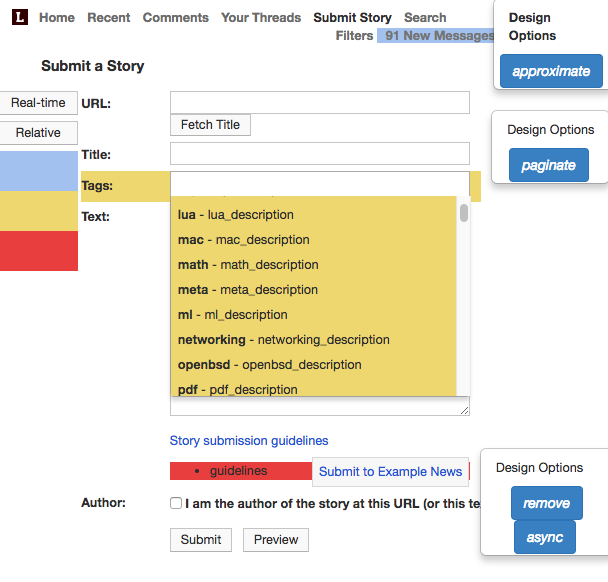
\includegraphics[width=\columnwidth]{panorama-figs/heatmap.png}
    \vspace{-0.1in}
    \caption{An example of \Tool browser interface}
    \label{fig:heatmap}
     \vspace{-0.2in}
\end{figure}

%Given the view-centric profiling (Section \ref{sec:profile}) and view-aware optimization  (Section \ref{sec:opt}) are available, 

\Tool comes with a new interface to present the cost estimation and optimization information, and help developers explore different web-page design options. We discuss the \Tool interface in this section.

%We have implemented our approach into a RubyMine  plugin.


\subsection{Information display in browser}
\label{sec:ide_browser}
\textbf{Showing view-centric cost estimation information.}
\Tool visualizes the performance information obtained by dynamic profiling or 
static estimation (Section \ref{sec:profile}) through a heat-map with the more costly
HTML element having a more red-ish background, as illustrated in
Figure \ref{fig:heatmap}.

To generate this heat map, \Tool reads the output of its 
view-centric cost estimation (Section \ref{sec:profile}) 
and creates a JavaScript file {\tt interactive.js} that 
sets the background color
of every HTML tag through
``{\tt \$(tag-id).css(``background-color'', color);}'', where {\tt tag-id} is the
unique HTML tag ID and {\tt color} is computed based on the cost estimation for this HTML tag (Section \ref{sec:profile}).
Web developers can choose to see different heat-maps with
buttons on the web page, like ``Real-time'' (dynamic profiling
results) and ``Relative'' (statically estimated results) 
in Figure \ref{fig:heatmap}. We set the color using the HSL color scheme, with
more expensive tags rendered with smaller hue values (i.e., more red-ish) and
cheaper tags with larger hue values (i.e., more blue-ish).
\iffalse
Hue represents the degree on the color wheel ranging from 0 to 360, 0 is red, 120 is green, and 240 is blue. We order the tags through their performance cost in the ascendant order, and get the total number of costs as N, then we calculate the color gradient as {\tt scale = 1.0 / (N - 1)}, and the color for tags in rank index will be 240 * (1 - i * scale). As a result, the larger the performance cost is, the HUE will be closer to 0 which means that it is be more red-ish, and the smaller the performance cost is, HUE will closer to 240 as known as more blue-ish.   
\fi


\iffalse 
\begin{figure}[h]
    \centering
    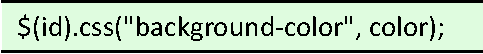
\includegraphics[width=\columnwidth]{figs/background.pdf}
    \caption{setting background color using javascript}
    \label{fig:bgchange}
\end{figure}
 \fi
 


\textbf{Showing view-aware optimization suggestions.}
%The JavaScript file created by \Tool above 
{\tt interactive.js} described above
helps display not only 
data-processing cost but
also alternative view-design options for various HTML tags. 
Users simply right click
an HTML tag in the browser to get a list of design options, as shown in Figure \ref{fig:heatmap}.
The implementation is straight-forward,
given the unique ID of every HTML tag and the performance-enhancing opportunities
identified through \Tool static analysis as discussed in Section \ref{sec:opt}.

\begin{figure}
    \centering
    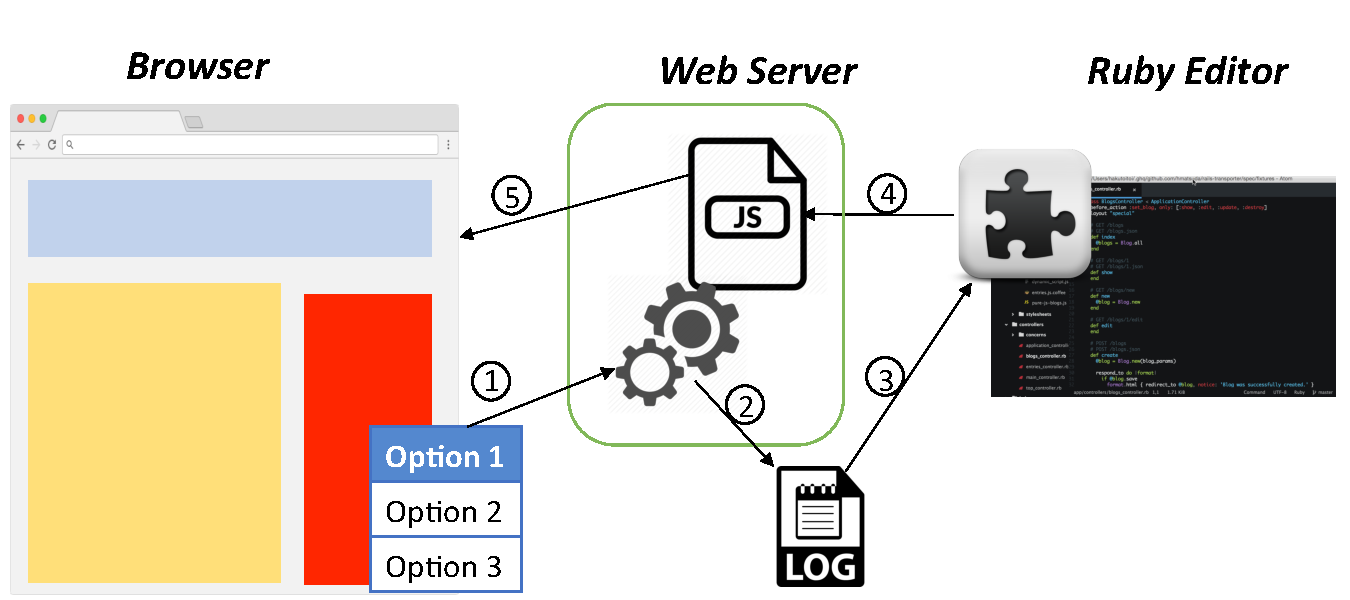
\includegraphics[width=\columnwidth]{panorama-figs/interface.pdf}
    \caption{\Tool interface implementation}
    \label{fig:interaction}
     \vspace{-0.2in}
\end{figure}

\subsection{Design-space exploration in browser}
To help developers explore different
performance--functionality design trade-offs, \Tool further
connects the browser-side information display and the Ruby editor side
refactoring together:
(1) developers first understand the data-processing cost 
of various HTML tags in the browser; 
(2) once developers choose an alternative design option for an HTML tag, 
the corresponding code refactoring will be automatically applied and displayed 
in the accompanying Ruby editor for developers to review; 
(3) once the source code is updated, the heat-map in the browser is
updated accordingly. Developers can explore different
design options, and eventually pick the best ones that suit their need.

To support this interface, \Tool carefully uses JavaScript, IDE plugin, and
other mechanisms
to help the communication between the browser and the Ruby editor, as illustrated
in Figure \ref{fig:interaction}.\footnote{The current prototype of \Tool assumes that the web-application under testing is deployed
on the same machine as the Ruby editor.}

First, \Tool automatically instruments the web application under development to help
communicate developers' design choices to the Ruby editor. Specifically, \Tool
adds a controller {\tt \_PANO\_handle\_request}
into the web application. Whenever developers click a design-option button,
like one of those blue {\it paginate}, {\it async}, {\it approximate},
{\it remove} buttons in Figure \ref{fig:heatmap}, 
\Tool
%the \Tool JavaScript file
%(i.e., the same one that creates the heat-map)
will send an HTTP request to invoke the {\tt \_PANO\_handle\_request} 
controller action ({\large \textcircled{\small 1}}  in Figure \ref{fig:interaction}), 
which then records the design-option type and the corresponding
HTML tag ID into a web-server side file {\tt request.log} ({\large \textcircled{\small 2}} in Figure \ref{fig:interaction}). 

In the editor, which we use RubyMine \cite{rubymine}, \Tool 
%creates an IDE plugin that 
uses a thread to monitor the {\tt request.log} file.
Whenever this file is changed, this monitoring thread will trigger the 
plugin to apply corresponding code refactoring in the IDE, with all the
code changes generated using algorithms described in Section \ref{sec:opt}
({\large \textcircled{\small 3}}  in Figure \ref{fig:interaction}). 

After the code change, the data-processing cost estimation will be updated automatically, which results in updates to a performance profile 
%{\tt log/development.log}
and corresponding updates to {\tt interactive.js} %\Tool JavaScript file
with changed background-color settings ({\large \textcircled{\small 4}}  
in Figure \ref{fig:interaction}).
%The changes in the JavaScript file will lead to 
The changes in {\tt interactive.js} lead to
an automated refresh in the browser with the updated heat-map display, as we use  the Ruby 
{\tt react-rails-hot-loader} to enable
automated refresh at every change in the Ruby source code or 
heat-map display code
%the \Tool JavaScript code 
({\large \textcircled{\small 5}}  in Figure \ref{fig:interaction}).



% Our current implementation using RubyMine \cite{rubymine}, one of the most popular Ruby on Rails
% IDE. \Tool's RubyMine plug-in uses
% IntelliJ APIs, like {\tt FileEditorManager}, {\tt TextRange}, and {\tt Document},
% to insert, replace, and delete source code in the code editor panel of RubyMine.  

